\documentclass[twoside]{book}

% Packages required by doxygen
\usepackage{fixltx2e}
\usepackage{calc}
\usepackage{doxygen}
\usepackage[export]{adjustbox} % also loads graphicx
\usepackage{graphicx}
\usepackage[utf8]{inputenc}
\usepackage{makeidx}
\usepackage{multicol}
\usepackage{multirow}
\PassOptionsToPackage{warn}{textcomp}
\usepackage{textcomp}
\usepackage[nointegrals]{wasysym}
\usepackage[table]{xcolor}

% Font selection
\usepackage[T1]{fontenc}
\usepackage[scaled=.90]{helvet}
\usepackage{courier}
\usepackage{amssymb}
\usepackage{sectsty}
\renewcommand{\familydefault}{\sfdefault}
\allsectionsfont{%
  \fontseries{bc}\selectfont%
  \color{darkgray}%
}
\renewcommand{\DoxyLabelFont}{%
  \fontseries{bc}\selectfont%
  \color{darkgray}%
}
\newcommand{\+}{\discretionary{\mbox{\scriptsize$\hookleftarrow$}}{}{}}

% Page & text layout
\usepackage{geometry}
\geometry{%
  a4paper,%
  top=2.5cm,%
  bottom=2.5cm,%
  left=2.5cm,%
  right=2.5cm%
}
\tolerance=750
\hfuzz=15pt
\hbadness=750
\setlength{\emergencystretch}{15pt}
\setlength{\parindent}{0cm}
\setlength{\parskip}{0.2cm}
\makeatletter
\renewcommand{\paragraph}{%
  \@startsection{paragraph}{4}{0ex}{-1.0ex}{1.0ex}{%
    \normalfont\normalsize\bfseries\SS@parafont%
  }%
}
\renewcommand{\subparagraph}{%
  \@startsection{subparagraph}{5}{0ex}{-1.0ex}{1.0ex}{%
    \normalfont\normalsize\bfseries\SS@subparafont%
  }%
}
\makeatother

% Headers & footers
\usepackage{fancyhdr}
\pagestyle{fancyplain}
\fancyhead[LE]{\fancyplain{}{\bfseries\thepage}}
\fancyhead[CE]{\fancyplain{}{}}
\fancyhead[RE]{\fancyplain{}{\bfseries\leftmark}}
\fancyhead[LO]{\fancyplain{}{\bfseries\rightmark}}
\fancyhead[CO]{\fancyplain{}{}}
\fancyhead[RO]{\fancyplain{}{\bfseries\thepage}}
\fancyfoot[LE]{\fancyplain{}{}}
\fancyfoot[CE]{\fancyplain{}{}}
\fancyfoot[RE]{\fancyplain{}{\bfseries\scriptsize Generated on Fri May 6 2016 21\+:40\+:47 for my\+G\+L by Doxygen }}
\fancyfoot[LO]{\fancyplain{}{\bfseries\scriptsize Generated on Fri May 6 2016 21\+:40\+:47 for my\+G\+L by Doxygen }}
\fancyfoot[CO]{\fancyplain{}{}}
\fancyfoot[RO]{\fancyplain{}{}}
\renewcommand{\footrulewidth}{0.4pt}
\renewcommand{\chaptermark}[1]{%
  \markboth{#1}{}%
}
\renewcommand{\sectionmark}[1]{%
  \markright{\thesection\ #1}%
}

% Indices & bibliography
\usepackage{natbib}
\usepackage[titles]{tocloft}
\setcounter{tocdepth}{3}
\setcounter{secnumdepth}{5}
\makeindex

% Hyperlinks (required, but should be loaded last)
\usepackage{ifpdf}
\ifpdf
  \usepackage[pdftex,pagebackref=true]{hyperref}
\else
  \usepackage[ps2pdf,pagebackref=true]{hyperref}
\fi
\hypersetup{%
  colorlinks=true,%
  linkcolor=blue,%
  citecolor=blue,%
  unicode%
}

% Custom commands
\newcommand{\clearemptydoublepage}{%
  \newpage{\pagestyle{empty}\cleardoublepage}%
}


%===== C O N T E N T S =====

\begin{document}

% Titlepage & ToC
\hypersetup{pageanchor=false,
             bookmarks=true,
             bookmarksnumbered=true,
             pdfencoding=unicode
            }
\pagenumbering{roman}
\begin{titlepage}
\vspace*{7cm}
\begin{center}%
{\Large my\+G\+L }\\
\vspace*{1cm}
{\large Generated by Doxygen 1.8.9.1}\\
\vspace*{0.5cm}
{\small Fri May 6 2016 21:40:47}\\
\end{center}
\end{titlepage}
\clearemptydoublepage
\tableofcontents
\clearemptydoublepage
\pagenumbering{arabic}
\hypersetup{pageanchor=true}

%--- Begin generated contents ---
\chapter{Hierarchical Index}
\section{Class Hierarchy}
This inheritance list is sorted roughly, but not completely, alphabetically\+:\begin{DoxyCompactList}
\item \contentsline{section}{args}{\pageref{structargs}}{}
\item \contentsline{section}{arguments}{\pageref{structarguments}}{}
\item \contentsline{section}{Context}{\pageref{classContext}}{}
\begin{DoxyCompactList}
\item \contentsline{section}{Composer}{\pageref{classComposer}}{}
\end{DoxyCompactList}
\item \contentsline{section}{Input}{\pageref{classInput}}{}
\begin{DoxyCompactList}
\item \contentsline{section}{Cursor\+Movement}{\pageref{classCursorMovement}}{}
\item \contentsline{section}{Key}{\pageref{classKey}}{}
\item \contentsline{section}{Mouse\+Button}{\pageref{classMouseButton}}{}
\end{DoxyCompactList}
\item \contentsline{section}{P\+NG}{\pageref{classPNG}}{}
\item \contentsline{section}{Shader\+Program}{\pageref{classShaderProgram}}{}
\item \contentsline{section}{shader\+Uniforms}{\pageref{structshaderUniforms}}{}
\item \contentsline{section}{Shape}{\pageref{classShape}}{}
\begin{DoxyCompactList}
\item \contentsline{section}{Line}{\pageref{classLine}}{}
\item \contentsline{section}{Rectangle}{\pageref{classRectangle}}{}
\end{DoxyCompactList}
\item \contentsline{section}{View}{\pageref{classView}}{}
\end{DoxyCompactList}

\chapter{Class Index}
\section{Class List}
Here are the classes, structs, unions and interfaces with brief descriptions\+:\begin{DoxyCompactList}
\item\contentsline{section}{\hyperlink{structargs}{args} }{\pageref{structargs}}{}
\item\contentsline{section}{\hyperlink{classContext}{Context} }{\pageref{classContext}}{}
\item\contentsline{section}{\hyperlink{classCursorMovement}{Cursor\+Movement} }{\pageref{classCursorMovement}}{}
\item\contentsline{section}{\hyperlink{classInput}{Input} }{\pageref{classInput}}{}
\item\contentsline{section}{\hyperlink{classKey}{Key} }{\pageref{classKey}}{}
\item\contentsline{section}{\hyperlink{classMouseButton}{Mouse\+Button} }{\pageref{classMouseButton}}{}
\item\contentsline{section}{\hyperlink{classMyGL}{My\+GL} }{\pageref{classMyGL}}{}
\item\contentsline{section}{\hyperlink{classPNG}{P\+NG} }{\pageref{classPNG}}{}
\item\contentsline{section}{\hyperlink{classShaderProgram}{Shader\+Program} }{\pageref{classShaderProgram}}{}
\item\contentsline{section}{\hyperlink{classShaderTextured}{Shader\+Textured} }{\pageref{classShaderTextured}}{}
\item\contentsline{section}{\hyperlink{classShape}{Shape} }{\pageref{classShape}}{}
\item\contentsline{section}{\hyperlink{classView}{View} }{\pageref{classView}}{}
\item\contentsline{section}{\hyperlink{classWindow}{Window} }{\pageref{classWindow}}{}
\item\contentsline{section}{\hyperlink{structWindowHints}{Window\+Hints} }{\pageref{structWindowHints}}{}
\end{DoxyCompactList}

\chapter{Class Documentation}
\hypertarget{structargs}{}\section{args Struct Reference}
\label{structargs}\index{args@{args}}
\subsection*{Public Types}
\begin{DoxyCompactItemize}
\item 
\hypertarget{structargs_a54c5a3a643a74c2e0dba4a3b8061d3e7}{}enum \{ {\bfseries A}, 
{\bfseries B}
 \}\label{structargs_a54c5a3a643a74c2e0dba4a3b8061d3e7}

\end{DoxyCompactItemize}
\subsection*{Public Attributes}
\begin{DoxyCompactItemize}
\item 
\hypertarget{structargs_a02a35dd00d558011e5c80e4b5083c649}{}enum args\+:: \{ ... \}  {\bfseries type}\label{structargs_a02a35dd00d558011e5c80e4b5083c649}

\item 
\hypertarget{structargs_a28ad94ec1e5034e6ce9a4d6be87475a0}{}\begin{tabbing}
xx\=xx\=xx\=xx\=xx\=xx\=xx\=xx\=xx\=\kill
union \{\\
\hypertarget{unionargs_1_1@1_afa6d8f0e9d79cc4603ad642ce19f883f}{}\>struct \{\\
\>\>int {\bfseries x}\\
\>\>int {\bfseries y}\\
\>\} \label{unionargs_1_1@1_afa6d8f0e9d79cc4603ad642ce19f883f}
\\
\hypertarget{unionargs_1_1@1_af071bca0f9407cbbf397f73a9e66ee60}{}\>struct \{\\
\>\>double {\bfseries z}\\
\>\} \label{unionargs_1_1@1_af071bca0f9407cbbf397f73a9e66ee60}
\\
\}; \label{structargs_a28ad94ec1e5034e6ce9a4d6be87475a0}
\\

\end{tabbing}\end{DoxyCompactItemize}


The documentation for this struct was generated from the following file\+:\begin{DoxyCompactItemize}
\item 
function\+Pointer\+Test.\+cpp\end{DoxyCompactItemize}

\hypertarget{classContext}{}\section{Context Class Reference}
\label{classContext}\index{Context@{Context}}


Inheritance diagram for Context\+:
\nopagebreak
\begin{figure}[H]
\begin{center}
\leavevmode
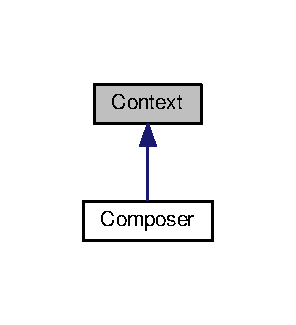
\includegraphics[width=142pt]{classContext__inherit__graph}
\end{center}
\end{figure}


Collaboration diagram for Context\+:
\nopagebreak
\begin{figure}[H]
\begin{center}
\leavevmode
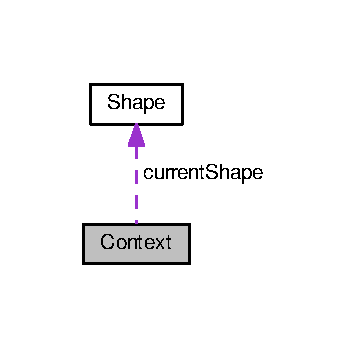
\includegraphics[width=217pt]{classContext__coll__graph}
\end{center}
\end{figure}
\subsection*{Public Member Functions}
\begin{DoxyCompactItemize}
\item 
\hypertarget{classContext_aa940262b2ab80eea625f768f0b6fac7a}{}virtual void {\bfseries cursor\+Movement} (\hyperlink{classCursorMovement}{Cursor\+Movement})=0\label{classContext_aa940262b2ab80eea625f768f0b6fac7a}

\item 
\hypertarget{classContext_a70da8923b6a5a138d8603c609bc31fa6}{}virtual void {\bfseries key} (\hyperlink{classKey}{Key})=0\label{classContext_a70da8923b6a5a138d8603c609bc31fa6}

\item 
\hypertarget{classContext_a3999d157f67e3ba18cd704a5d4f0178a}{}void {\bfseries mouse\+Button} (\hyperlink{classMouseButton}{Mouse\+Button})\label{classContext_a3999d157f67e3ba18cd704a5d4f0178a}

\item 
virtual void \hyperlink{classContext_ab47a1f761c1408d246ef99159b197d3a}{mb} (\hyperlink{classMouseButton}{Mouse\+Button})=0
\item 
\hypertarget{classContext_a8fb1191127d9d8b5d7c356fc62189d9a}{}virtual void {\bfseries render} ()=0\label{classContext_a8fb1191127d9d8b5d7c356fc62189d9a}

\end{DoxyCompactItemize}
\subsection*{Public Attributes}
\begin{DoxyCompactItemize}
\item 
\hypertarget{classContext_a16b34e7c1aae337963724ec597e4750d}{}\hyperlink{classContext}{Context} $\ast$ {\bfseries current\+Context}\label{classContext_a16b34e7c1aae337963724ec597e4750d}

\item 
\hypertarget{classContext_af2a331132fbccf0a841f1f9ba47d4203}{}int {\bfseries last\+Scancode}\label{classContext_af2a331132fbccf0a841f1f9ba47d4203}

\item 
\hypertarget{classContext_ac3e36ee8fc5f660558345e72149a56ab}{}bool {\bfseries mouse\+Pressed}\label{classContext_ac3e36ee8fc5f660558345e72149a56ab}

\end{DoxyCompactItemize}


\subsection{Member Function Documentation}
\hypertarget{classContext_ab47a1f761c1408d246ef99159b197d3a}{}\index{Context@{Context}!mb@{mb}}
\index{mb@{mb}!Context@{Context}}
\subsubsection[{mb}]{\setlength{\rightskip}{0pt plus 5cm}virtual void Context\+::mb (
\begin{DoxyParamCaption}
\item[{{\bf Mouse\+Button}}]{}
\end{DoxyParamCaption}
)\hspace{0.3cm}{\ttfamily [pure virtual]}}\label{classContext_ab47a1f761c1408d246ef99159b197d3a}
updates \textquotesingle{}mouse\+Pressed\textquotesingle{} before calling \hyperlink{classContext_ab47a1f761c1408d246ef99159b197d3a}{mb()} 

Implemented in \hyperlink{classComposer_aeccddfa85500c2e3a517058611ccca6a}{Composer}.



The documentation for this class was generated from the following files\+:\begin{DoxyCompactItemize}
\item 
my\+G\+L.\+hpp\item 
context.\+cpp\end{DoxyCompactItemize}

\hypertarget{classCursorMovement}{}\section{Cursor\+Movement Class Reference}
\label{classCursorMovement}\index{Cursor\+Movement@{Cursor\+Movement}}


Inheritance diagram for Cursor\+Movement\+:
\nopagebreak
\begin{figure}[H]
\begin{center}
\leavevmode
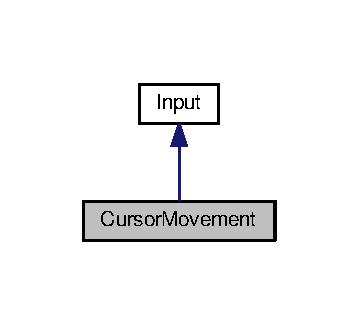
\includegraphics[width=172pt]{classCursorMovement__inherit__graph}
\end{center}
\end{figure}


Collaboration diagram for Cursor\+Movement\+:
\nopagebreak
\begin{figure}[H]
\begin{center}
\leavevmode
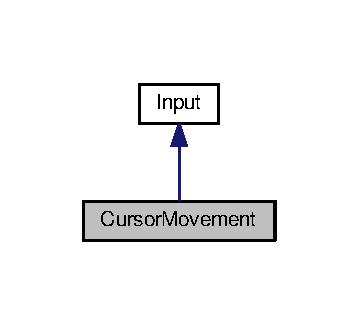
\includegraphics[width=172pt]{classCursorMovement__coll__graph}
\end{center}
\end{figure}
\subsection*{Public Member Functions}
\begin{DoxyCompactItemize}
\item 
{\bfseries Cursor\+Movement} (double xpos, double ypos)\hypertarget{classCursorMovement_a5d4ae67fcfe792baff996121b694e7c3}{}\label{classCursorMovement_a5d4ae67fcfe792baff996121b694e7c3}

\end{DoxyCompactItemize}
\subsection*{Public Attributes}
\begin{DoxyCompactItemize}
\item 
double {\bfseries x}\hypertarget{classCursorMovement_ac77861debf3dc2013b7ee0f6775b6540}{}\label{classCursorMovement_ac77861debf3dc2013b7ee0f6775b6540}

\item 
double {\bfseries y}\hypertarget{classCursorMovement_afab93e8fcc9f845fdcf6fffdf9232cab}{}\label{classCursorMovement_afab93e8fcc9f845fdcf6fffdf9232cab}

\end{DoxyCompactItemize}


The documentation for this class was generated from the following file\+:\begin{DoxyCompactItemize}
\item 
My\+G\+L.\+hpp\end{DoxyCompactItemize}

\hypertarget{classInput}{}\section{Input Class Reference}
\label{classInput}\index{Input@{Input}}


{\ttfamily \#include $<$my\+G\+L.\+hpp$>$}



Inheritance diagram for Input\+:
\nopagebreak
\begin{figure}[H]
\begin{center}
\leavevmode
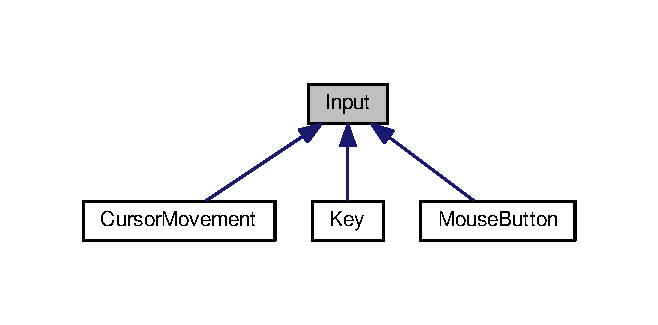
\includegraphics[width=316pt]{classInput__inherit__graph}
\end{center}
\end{figure}


\subsection{Detailed Description}
The member variables of \hyperlink{classCursorMovement}{Cursor\+Movement}, \hyperlink{classMouseButton}{Mouse\+Button}, and \hyperlink{classKey}{Key} match what is provided in the respective G\+L\+F\+W callback functions. 

The documentation for this class was generated from the following file\+:\begin{DoxyCompactItemize}
\item 
my\+G\+L.\+hpp\end{DoxyCompactItemize}

\hypertarget{classKey}{}\section{Key Class Reference}
\label{classKey}\index{Key@{Key}}


Inheritance diagram for Key\+:
\nopagebreak
\begin{figure}[H]
\begin{center}
\leavevmode
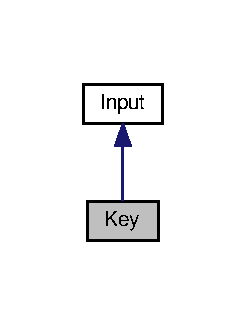
\includegraphics[width=118pt]{classKey__inherit__graph}
\end{center}
\end{figure}


Collaboration diagram for Key\+:
\nopagebreak
\begin{figure}[H]
\begin{center}
\leavevmode
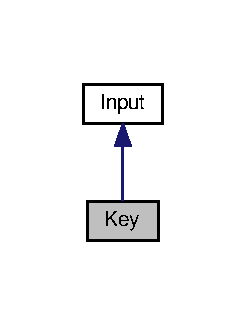
\includegraphics[width=118pt]{classKey__coll__graph}
\end{center}
\end{figure}
\subsection*{Public Member Functions}
\begin{DoxyCompactItemize}
\item 
{\bfseries Key} (int key, int scancode, int action, int mods)\hypertarget{classKey_a21c1c991388635db9b0690de6ff3292a}{}\label{classKey_a21c1c991388635db9b0690de6ff3292a}

\end{DoxyCompactItemize}
\subsection*{Public Attributes}
\begin{DoxyCompactItemize}
\item 
int {\bfseries key}\hypertarget{classKey_a49ddb6c986197664f6939db5dfd9c244}{}\label{classKey_a49ddb6c986197664f6939db5dfd9c244}

\item 
int {\bfseries scancode}\hypertarget{classKey_a13cb660e3e0d92129eeeaa56c5cc8296}{}\label{classKey_a13cb660e3e0d92129eeeaa56c5cc8296}

\item 
int {\bfseries action}\hypertarget{classKey_add8acc14210865bd9959bf38ee4e82f8}{}\label{classKey_add8acc14210865bd9959bf38ee4e82f8}

\item 
int {\bfseries mods}\hypertarget{classKey_a0e3f757c5b28ee99c9bf6f07811e6637}{}\label{classKey_a0e3f757c5b28ee99c9bf6f07811e6637}

\end{DoxyCompactItemize}


The documentation for this class was generated from the following file\+:\begin{DoxyCompactItemize}
\item 
My\+G\+L.\+hpp\end{DoxyCompactItemize}

\hypertarget{classMouseButton}{}\section{Mouse\+Button Class Reference}
\label{classMouseButton}\index{Mouse\+Button@{Mouse\+Button}}


Inheritance diagram for Mouse\+Button\+:
\nopagebreak
\begin{figure}[H]
\begin{center}
\leavevmode
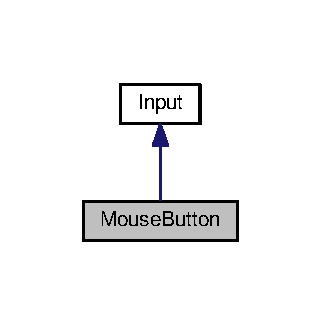
\includegraphics[width=154pt]{classMouseButton__inherit__graph}
\end{center}
\end{figure}


Collaboration diagram for Mouse\+Button\+:
\nopagebreak
\begin{figure}[H]
\begin{center}
\leavevmode
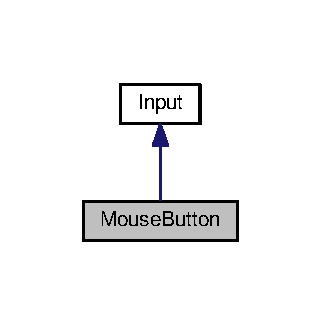
\includegraphics[width=154pt]{classMouseButton__coll__graph}
\end{center}
\end{figure}
\subsection*{Public Member Functions}
\begin{DoxyCompactItemize}
\item 
\hypertarget{classMouseButton_ad2a2ab9c8a5d0a95bae134566462136c}{}{\bfseries Mouse\+Button} (int button, int action, int mods)\label{classMouseButton_ad2a2ab9c8a5d0a95bae134566462136c}

\end{DoxyCompactItemize}
\subsection*{Public Attributes}
\begin{DoxyCompactItemize}
\item 
\hypertarget{classMouseButton_ada6d6e1d81eaedf7092a8617af6ede6b}{}int {\bfseries button}\label{classMouseButton_ada6d6e1d81eaedf7092a8617af6ede6b}

\item 
\hypertarget{classMouseButton_a7f22ddcecc4bfe282f7c8b150e28704b}{}int {\bfseries action}\label{classMouseButton_a7f22ddcecc4bfe282f7c8b150e28704b}

\item 
\hypertarget{classMouseButton_a1fa333819593583ccc090db9330018ad}{}int {\bfseries mods}\label{classMouseButton_a1fa333819593583ccc090db9330018ad}

\end{DoxyCompactItemize}


The documentation for this class was generated from the following file\+:\begin{DoxyCompactItemize}
\item 
my\+G\+L.\+hpp\end{DoxyCompactItemize}

\hypertarget{classMyGL}{}\section{My\+G\+L Class Reference}
\label{classMyGL}\index{My\+G\+L@{My\+G\+L}}


{\ttfamily \#include $<$My\+G\+L.\+hpp$>$}



Collaboration diagram for My\+G\+L\+:
\nopagebreak
\begin{figure}[H]
\begin{center}
\leavevmode
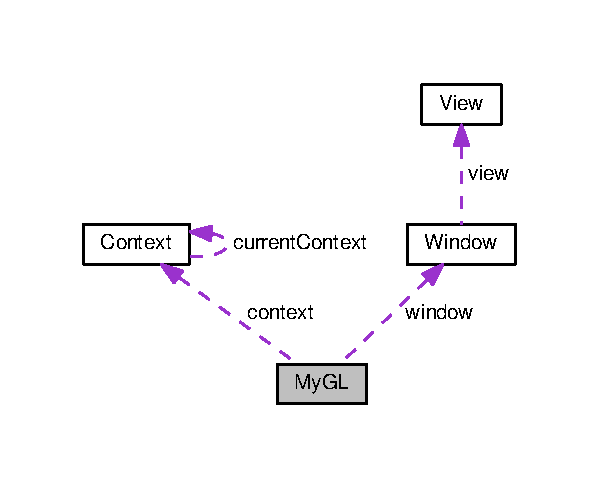
\includegraphics[width=307pt]{classMyGL__coll__graph}
\end{center}
\end{figure}
\subsection*{Public Member Functions}
\begin{DoxyCompactItemize}
\item 
\hyperlink{classMyGL_abb621dca31a152540b416deadf23037c}{My\+G\+L} ()
\item 
void \hyperlink{classMyGL_a4c37ec888e514cc8d06b7bc0ea7e73bd}{main\+Loop} ()
\item 
void \hyperlink{classMyGL_af7fa10909864af7f8417cf12553ba456}{gen\+Lots\+Windows} ()
\item 
G\+L\+F\+Wwindow $\ast$ \hyperlink{classMyGL_a9f2cc53d2c05eceb1d433bb0b19d9db8}{make\+Window\+For\+Context} ()
\end{DoxyCompactItemize}
\subsection*{Public Attributes}
\begin{DoxyCompactItemize}
\item 
\hypertarget{classMyGL_ad9da207aec683d4e52190aa6ca4c8103}{}G\+L\+F\+Wwindow $\ast$ {\bfseries window\+For\+Context}\label{classMyGL_ad9da207aec683d4e52190aa6ca4c8103}

\item 
\hypertarget{classMyGL_a64f2144f0057b9b37b14ebc9a94d4f75}{}\hyperlink{classContext}{Context} $\ast$ {\bfseries current\+Context}\label{classMyGL_a64f2144f0057b9b37b14ebc9a94d4f75}

\item 
\hypertarget{classMyGL_ae0a53010a55ec6920697018b90df6ee2}{}\hyperlink{classShaderProgram}{Shader\+Program} $\ast$ {\bfseries current\+Shader\+Program}\label{classMyGL_ae0a53010a55ec6920697018b90df6ee2}

\item 
\hypertarget{classMyGL_ab7bc049b7ce8d79fe244a1dbd2e63bf0}{}std\+::list$<$ \hyperlink{classWindow}{Window} $\ast$ $>$ {\bfseries windows}\label{classMyGL_ab7bc049b7ce8d79fe244a1dbd2e63bf0}

\item 
\hypertarget{classMyGL_a349d4b9d76a0427c048ab86c75346c8f}{}std\+::vector$<$ std\+::unique\+\_\+ptr$<$ \hyperlink{classContext}{Context} $>$ $>$ {\bfseries contexts}\label{classMyGL_a349d4b9d76a0427c048ab86c75346c8f}

\item 
\hypertarget{classMyGL_ad538dbfd1535c800bb09cab39e85226b}{}std\+::vector$<$ std\+::unique\+\_\+ptr$<$ \hyperlink{classShaderProgram}{Shader\+Program} $>$ $>$ {\bfseries shader\+Programs}\label{classMyGL_ad538dbfd1535c800bb09cab39e85226b}

\item 
\hypertarget{classMyGL_ae9b56982144e61ad3cdbd1941ece779c}{}std\+::string {\bfseries vertex\+Shader\+File\+Name} \{\char`\"{}vertex\+Shader.\+glsl\char`\"{}\}\label{classMyGL_ae9b56982144e61ad3cdbd1941ece779c}

\item 
\hypertarget{classMyGL_a8366fc1559f38d409baefeb5df9a1d59}{}std\+::string {\bfseries fragment\+Shader\+File\+Name} \{\char`\"{}fragment\+Shader.\+glsl\char`\"{}\}\label{classMyGL_a8366fc1559f38d409baefeb5df9a1d59}

\end{DoxyCompactItemize}


\subsection{Detailed Description}
This is the topmost class for the program. Creating a new instance of this class means creating a new instance of the program. The main program should be as simple as running My\+G\+L$\ast$ mygl = new \hyperlink{classMyGL_abb621dca31a152540b416deadf23037c}{My\+G\+L()}; The main.\+cpp main can then interact with the program in different ways through mygl. mygl-\/$>$get\+Current\+Context(); mygl-\/$>$switch\+Current\+Context(\+Context); 

\subsection{Constructor \& Destructor Documentation}
\hypertarget{classMyGL_abb621dca31a152540b416deadf23037c}{}\index{My\+G\+L@{My\+G\+L}!My\+G\+L@{My\+G\+L}}
\index{My\+G\+L@{My\+G\+L}!My\+G\+L@{My\+G\+L}}
\subsubsection[{My\+G\+L}]{\setlength{\rightskip}{0pt plus 5cm}My\+G\+L\+::\+My\+G\+L (
\begin{DoxyParamCaption}
{}
\end{DoxyParamCaption}
)}\label{classMyGL_abb621dca31a152540b416deadf23037c}
Initialize the library 

\subsection{Member Function Documentation}
\hypertarget{classMyGL_af7fa10909864af7f8417cf12553ba456}{}\index{My\+G\+L@{My\+G\+L}!gen\+Lots\+Windows@{gen\+Lots\+Windows}}
\index{gen\+Lots\+Windows@{gen\+Lots\+Windows}!My\+G\+L@{My\+G\+L}}
\subsubsection[{gen\+Lots\+Windows}]{\setlength{\rightskip}{0pt plus 5cm}void My\+G\+L\+::gen\+Lots\+Windows (
\begin{DoxyParamCaption}
{}
\end{DoxyParamCaption}
)}\label{classMyGL_af7fa10909864af7f8417cf12553ba456}
Calls on all the windows to update themselvs. \hypertarget{classMyGL_a4c37ec888e514cc8d06b7bc0ea7e73bd}{}\index{My\+G\+L@{My\+G\+L}!main\+Loop@{main\+Loop}}
\index{main\+Loop@{main\+Loop}!My\+G\+L@{My\+G\+L}}
\subsubsection[{main\+Loop}]{\setlength{\rightskip}{0pt plus 5cm}void My\+G\+L\+::main\+Loop (
\begin{DoxyParamCaption}
{}
\end{DoxyParamCaption}
)}\label{classMyGL_a4c37ec888e514cc8d06b7bc0ea7e73bd}
If the thread has finished then we assume the window do have destructed. We just erase the unique\+\_\+ptr from the list. \hypertarget{classMyGL_a9f2cc53d2c05eceb1d433bb0b19d9db8}{}\index{My\+G\+L@{My\+G\+L}!make\+Window\+For\+Context@{make\+Window\+For\+Context}}
\index{make\+Window\+For\+Context@{make\+Window\+For\+Context}!My\+G\+L@{My\+G\+L}}
\subsubsection[{make\+Window\+For\+Context}]{\setlength{\rightskip}{0pt plus 5cm}G\+L\+F\+Wwindow $\ast$ My\+G\+L\+::make\+Window\+For\+Context (
\begin{DoxyParamCaption}
{}
\end{DoxyParamCaption}
)}\label{classMyGL_a9f2cc53d2c05eceb1d433bb0b19d9db8}
for mac compatability 

The documentation for this class was generated from the following files\+:\begin{DoxyCompactItemize}
\item 
My\+G\+L.\+hpp\item 
My\+G\+L.\+cpp\end{DoxyCompactItemize}

\hypertarget{classPNG}{}\section{P\+NG Class Reference}
\label{classPNG}\index{P\+NG@{P\+NG}}


{\ttfamily \#include $<$my\+G\+L.\+hpp$>$}

\subsection*{Public Member Functions}
\begin{DoxyCompactItemize}
\item 
{\bfseries P\+NG} (char image\+Name\mbox{[}$\,$\mbox{]})\hypertarget{classPNG_a8239ef58cce7dfa23bf02a7620e985f5}{}\label{classPNG_a8239ef58cce7dfa23bf02a7620e985f5}

\item 
void {\bfseries read} ()\hypertarget{classPNG_a48b56be2d085e01f01b140528f999f5b}{}\label{classPNG_a48b56be2d085e01f01b140528f999f5b}

\item 
void {\bfseries write} ()\hypertarget{classPNG_a3e0b622c7ab188c3024295f8eebedd04}{}\label{classPNG_a3e0b622c7ab188c3024295f8eebedd04}

\item 
int {\bfseries width} ()\hypertarget{classPNG_a2b1a554b4f86d1b8ffa07c298782b14d}{}\label{classPNG_a2b1a554b4f86d1b8ffa07c298782b14d}

\item 
int {\bfseries height} ()\hypertarget{classPNG_ad6f6685a921c0f26352e22dc144fdda6}{}\label{classPNG_ad6f6685a921c0f26352e22dc144fdda6}

\item 
unsigned char $\ast$ {\bfseries pixels} ()\hypertarget{classPNG_a07898bac65710ae8aaeea6048dc773bc}{}\label{classPNG_a07898bac65710ae8aaeea6048dc773bc}

\end{DoxyCompactItemize}
\subsection*{Static Public Member Functions}
\begin{DoxyCompactItemize}
\item 
static unsigned char $\ast$ {\bfseries read\+P\+NG} (char $\ast$image\+Name)\hypertarget{classPNG_a6df04a0372aa1054cc85a219829d882a}{}\label{classPNG_a6df04a0372aa1054cc85a219829d882a}

\item 
static void {\bfseries write\+P\+NG} (char image\+Name\mbox{[}$\,$\mbox{]}, unsigned char $\ast$data, int width, int height)\hypertarget{classPNG_a12fe7f480b617e0cd58bd0ca7a65ed3a}{}\label{classPNG_a12fe7f480b617e0cd58bd0ca7a65ed3a}

\end{DoxyCompactItemize}
\subsection*{Public Attributes}
\begin{DoxyCompactItemize}
\item 
png\+\_\+image {\bfseries image}\hypertarget{classPNG_adcccee60854d7ef75c4f516b26d9be7e}{}\label{classPNG_adcccee60854d7ef75c4f516b26d9be7e}

\item 
char $\ast$ {\bfseries image\+Name}\hypertarget{classPNG_af06d37031363a6e28cd16cde17fe87bf}{}\label{classPNG_af06d37031363a6e28cd16cde17fe87bf}

\item 
unsigned char $\ast$ {\bfseries data}\hypertarget{classPNG_af96e0999d0c4b3fb0219462daf297d92}{}\label{classPNG_af96e0999d0c4b3fb0219462daf297d92}

\end{DoxyCompactItemize}


\subsection{Detailed Description}
The \hyperlink{classPNG}{P\+NG} class is for reading and writing \textquotesingle{}.png\textquotesingle{} files. There are two static functions called read\+P\+N\+G() and write\+P\+N\+G() that can be used without instantiating an instance of the class. This class was made to solve the problem that write\+P\+N\+G(read\+P\+N\+G(file\+Name)); write\+P\+NG in the above statement doesn\textquotesingle{}t know the width and height of the image. Now the width and height are stored in the object itself. 

The documentation for this class was generated from the following files\+:\begin{DoxyCompactItemize}
\item 
my\+G\+L.\+hpp\item 
context.\+cpp\end{DoxyCompactItemize}

\hypertarget{classShaderProgram}{}\section{Shader\+Program Class Reference}
\label{classShaderProgram}\index{Shader\+Program@{Shader\+Program}}


Inheritance diagram for Shader\+Program\+:
\nopagebreak
\begin{figure}[H]
\begin{center}
\leavevmode
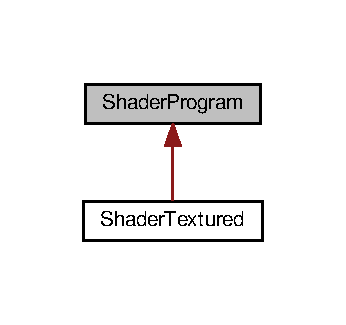
\includegraphics[width=166pt]{classShaderProgram__inherit__graph}
\end{center}
\end{figure}
\subsection*{Public Member Functions}
\begin{DoxyCompactItemize}
\item 
\hyperlink{classShaderProgram_a1ebd997652d664bb4cfad4327dfc0ebf}{Shader\+Program} (std\+::string vertex\+Shader\+File\+Name, std\+::string fragment\+Shader\+File\+Name)
\item 
\hypertarget{classShaderProgram_a266426e0200266b6776e8a5a8b1506b0}{}void {\bfseries check\+Shader\+Step\+Success} (G\+Luint shader, G\+Luint status)\label{classShaderProgram_a266426e0200266b6776e8a5a8b1506b0}

\item 
\hypertarget{classShaderProgram_ab9aaa0cdb43bd9de8a370e2869354a8a}{}void {\bfseries print\+Shader\+Log} (char $\ast$error\+Message, G\+Luint shader)\label{classShaderProgram_ab9aaa0cdb43bd9de8a370e2869354a8a}

\item 
\hypertarget{classShaderProgram_a190a33eec6ed3138a6d94a7305a9e831}{}G\+Luint {\bfseries id} ()\label{classShaderProgram_a190a33eec6ed3138a6d94a7305a9e831}

\end{DoxyCompactItemize}
\subsection*{Static Public Member Functions}
\begin{DoxyCompactItemize}
\item 
\hypertarget{classShaderProgram_ab0705c01246e6a70e8c3bc278666b2d0}{}static std\+::string {\bfseries read\+File} (std\+::string file\+Name)\label{classShaderProgram_ab0705c01246e6a70e8c3bc278666b2d0}

\end{DoxyCompactItemize}
\subsection*{Public Attributes}
\begin{DoxyCompactItemize}
\item 
\hypertarget{classShaderProgram_a5cd33e7bf1c9d23b2eef8aa93dc36558}{}G\+Luint {\bfseries program}\label{classShaderProgram_a5cd33e7bf1c9d23b2eef8aa93dc36558}

\item 
\hypertarget{classShaderProgram_ad9000af8292a5de7a33108ae6c775acd}{}G\+Lint {\bfseries view\+Offset\+X}\label{classShaderProgram_ad9000af8292a5de7a33108ae6c775acd}

\item 
\hypertarget{classShaderProgram_a5f68b35bbd45e69c2b53310cc5f6d73f}{}G\+Lint {\bfseries view\+Offset\+Y}\label{classShaderProgram_a5f68b35bbd45e69c2b53310cc5f6d73f}

\item 
\hypertarget{classShaderProgram_ab228e6feb1db07d20255c6bde5ed33a8}{}G\+Lint {\bfseries units\+Per\+Pixel\+X}\label{classShaderProgram_ab228e6feb1db07d20255c6bde5ed33a8}

\item 
\hypertarget{classShaderProgram_addaecff211bcb14fe9f254c31f407327}{}G\+Lint {\bfseries units\+Per\+Pixel\+Y}\label{classShaderProgram_addaecff211bcb14fe9f254c31f407327}

\item 
\hypertarget{classShaderProgram_ac9dc87f9ae304100c66a86f59c6ddc63}{}G\+Lint {\bfseries screen\+Width}\label{classShaderProgram_ac9dc87f9ae304100c66a86f59c6ddc63}

\item 
\hypertarget{classShaderProgram_adf3cf91290d9ccdc9a07a88dffaf8bcb}{}G\+Lint {\bfseries screen\+Height}\label{classShaderProgram_adf3cf91290d9ccdc9a07a88dffaf8bcb}

\end{DoxyCompactItemize}


\subsection{Constructor \& Destructor Documentation}
\hypertarget{classShaderProgram_a1ebd997652d664bb4cfad4327dfc0ebf}{}\index{Shader\+Program@{Shader\+Program}!Shader\+Program@{Shader\+Program}}
\index{Shader\+Program@{Shader\+Program}!Shader\+Program@{Shader\+Program}}
\subsubsection[{Shader\+Program}]{\setlength{\rightskip}{0pt plus 5cm}Shader\+Program\+::\+Shader\+Program (
\begin{DoxyParamCaption}
\item[{std\+::string}]{vertex\+Shader\+File\+Name, }
\item[{std\+::string}]{fragment\+Shader\+File\+Name}
\end{DoxyParamCaption}
)}\label{classShaderProgram_a1ebd997652d664bb4cfad4327dfc0ebf}
Reads in a couple text files, compiles and links stuff and makes a shader program. Calls gl\+Use\+Program at the end and then needs to set up the uniforms. 

The documentation for this class was generated from the following files\+:\begin{DoxyCompactItemize}
\item 
My\+G\+L.\+hpp\item 
My\+G\+L.\+cpp\end{DoxyCompactItemize}

\hypertarget{classShaderTextured}{}\section{Shader\+Textured Class Reference}
\label{classShaderTextured}\index{Shader\+Textured@{Shader\+Textured}}


Inheritance diagram for Shader\+Textured\+:
\nopagebreak
\begin{figure}[H]
\begin{center}
\leavevmode
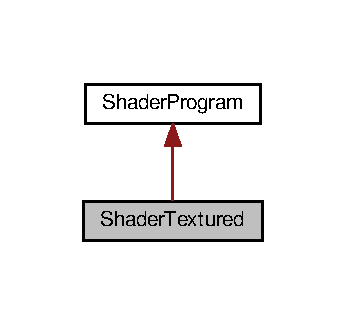
\includegraphics[width=166pt]{classShaderTextured__inherit__graph}
\end{center}
\end{figure}


Collaboration diagram for Shader\+Textured\+:
\nopagebreak
\begin{figure}[H]
\begin{center}
\leavevmode
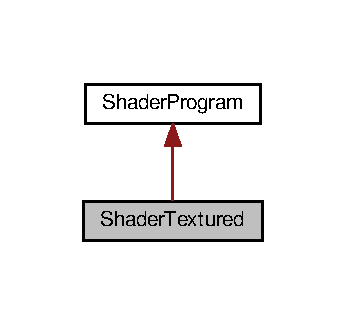
\includegraphics[width=166pt]{classShaderTextured__coll__graph}
\end{center}
\end{figure}


The documentation for this class was generated from the following file\+:\begin{DoxyCompactItemize}
\item 
My\+G\+L.\+hpp\end{DoxyCompactItemize}

\hypertarget{classShape}{}\section{Shape Class Reference}
\label{classShape}\index{Shape@{Shape}}


{\ttfamily \#include $<$My\+G\+L.\+hpp$>$}

\subsection*{Public Types}
\begin{DoxyCompactItemize}
\item 
\hypertarget{classShape_ab0227d9b119beea793bce34ba3e0b5b8}{}typedef void(Shape\+::$\ast$ {\bfseries render\+Func}) (void)\label{classShape_ab0227d9b119beea793bce34ba3e0b5b8}

\end{DoxyCompactItemize}
\subsection*{Public Member Functions}
\begin{DoxyCompactItemize}
\item 
\hypertarget{classShape_a1b3bc50a2d114a27f144a834e7f0af64}{}{\bfseries Shape} (float x, float y)\label{classShape_a1b3bc50a2d114a27f144a834e7f0af64}

\item 
\hypertarget{classShape_a0098f3d6067b650de0b5e34f44a9257f}{}int {\bfseries data\+Length} ()\label{classShape_a0098f3d6067b650de0b5e34f44a9257f}

\item 
\hypertarget{classShape_a3651abfa2b1d449f35c83b3dc64f64f2}{}void {\bfseries finish} ()\label{classShape_a3651abfa2b1d449f35c83b3dc64f64f2}

\item 
void \hyperlink{classShape_ad62ee6dbad795d967e2f572f6e4e27fb}{render} ()
\end{DoxyCompactItemize}


\subsection{Detailed Description}
The \hyperlink{classShape}{Shape} class allows a very nice vector$<$\+Shape$\ast$$>$ in \hyperlink{classContext}{Context}. The common stuff for rendering goes here. 

\subsection{Member Function Documentation}
\hypertarget{classShape_ad62ee6dbad795d967e2f572f6e4e27fb}{}\index{Shape@{Shape}!render@{render}}
\index{render@{render}!Shape@{Shape}}
\subsubsection[{render}]{\setlength{\rightskip}{0pt plus 5cm}void Shape\+::render (
\begin{DoxyParamCaption}
{}
\end{DoxyParamCaption}
)}\label{classShape_ad62ee6dbad795d967e2f572f6e4e27fb}
prep the data, gen the buffers, and make \textquotesingle{}render\+Ptr\textquotesingle{} point to \textquotesingle{}final\+Render\textquotesingle{} called before pushing the current shape onto context\textquotesingle{}s vector$<$\+Shape$\ast$$>$ 

The documentation for this class was generated from the following files\+:\begin{DoxyCompactItemize}
\item 
My\+G\+L.\+hpp\item 
My\+G\+L.\+cpp\end{DoxyCompactItemize}

\hypertarget{classView}{}\section{View Class Reference}
\label{classView}\index{View@{View}}


{\ttfamily \#include $<$My\+G\+L.\+hpp$>$}



Collaboration diagram for View\+:\nopagebreak
\begin{figure}[H]
\begin{center}
\leavevmode
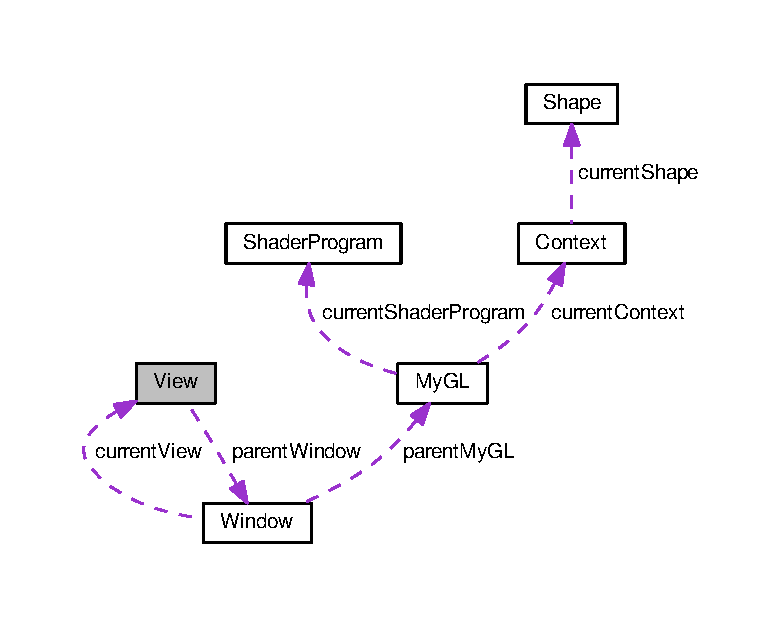
\includegraphics[width=350pt]{classView__coll__graph}
\end{center}
\end{figure}
\subsection*{Public Member Functions}
\begin{DoxyCompactItemize}
\item 
{\bfseries View} (\hyperlink{classWindow}{Window} $\ast$window, int width, int height)\hypertarget{classView_a8e2813e8beabcfee72e2ec2e05fd72bb}{}\label{classView_a8e2813e8beabcfee72e2ec2e05fd72bb}

\item 
void {\bfseries translate} (float x, float y)\hypertarget{classView_a2e97f6058d6a6690d9db72ceb43478a4}{}\label{classView_a2e97f6058d6a6690d9db72ceb43478a4}

\item 
void {\bfseries scale} (float num)\hypertarget{classView_ac31ae2aee1e5374df420b657b3040f6d}{}\label{classView_ac31ae2aee1e5374df420b657b3040f6d}

\item 
double {\bfseries pixel\+To\+RealX} (double px)\hypertarget{classView_ad6c9a0c29d23c21f333b346aa538472a}{}\label{classView_ad6c9a0c29d23c21f333b346aa538472a}

\item 
double {\bfseries pixel\+To\+RealY} (double py)\hypertarget{classView_adc37e8999407e00288c7ef8e36d7bea1}{}\label{classView_adc37e8999407e00288c7ef8e36d7bea1}

\end{DoxyCompactItemize}
\subsection*{Public Attributes}
\begin{DoxyCompactItemize}
\item 
\hyperlink{classWindow}{Window} $\ast$ {\bfseries parent\+Window}\hypertarget{classView_ae047212bfa12abf0f0a57bf604e020ba}{}\label{classView_ae047212bfa12abf0f0a57bf604e020ba}

\item 
int {\bfseries width}\hypertarget{classView_ae039aa744b085db819ae149705b2c32b}{}\label{classView_ae039aa744b085db819ae149705b2c32b}

\item 
int {\bfseries height}\hypertarget{classView_a6e3e5c18893617490f02166641356746}{}\label{classView_a6e3e5c18893617490f02166641356746}

\item 
double {\bfseries view\+OffsetX} = 0.\+0\hypertarget{classView_a9b210244771d77ebcc08e5f9e9862922}{}\label{classView_a9b210244771d77ebcc08e5f9e9862922}

\item 
double {\bfseries view\+OffsetY} = 0.\+0\hypertarget{classView_ae18f735f6c322277e5788fa56bb9c758}{}\label{classView_ae18f735f6c322277e5788fa56bb9c758}

\item 
double {\bfseries units\+Per\+PixelX} = 1.\+0\hypertarget{classView_ad2318a59fa2280eab8b7a59d317f4e5a}{}\label{classView_ad2318a59fa2280eab8b7a59d317f4e5a}

\item 
double {\bfseries units\+Per\+PixelY} = 1.\+0\hypertarget{classView_a28db7efdb0540ef7cdc49934ecb79893}{}\label{classView_a28db7efdb0540ef7cdc49934ecb79893}

\end{DoxyCompactItemize}


\subsection{Detailed Description}
A window has a view object. The \hyperlink{classView}{View} is responsible for maintaining the variables that the vertex\+Shader uses to translate the points from real space to apparent space. Real space refers to the reference by which all of the shape objects in the Composer context are saved. It stretches from -\/inf to +inf. Apparent space is the (-\/1, 1) clamped view recognised by opengl. 

The documentation for this class was generated from the following files\+:\begin{DoxyCompactItemize}
\item 
My\+G\+L.\+hpp\item 
My\+G\+L.\+cpp\end{DoxyCompactItemize}

\hypertarget{classWindow}{}\section{Window Class Reference}
\label{classWindow}\index{Window@{Window}}


{\ttfamily \#include $<$My\+G\+L.\+hpp$>$}



Collaboration diagram for Window\+:
\nopagebreak
\begin{figure}[H]
\begin{center}
\leavevmode
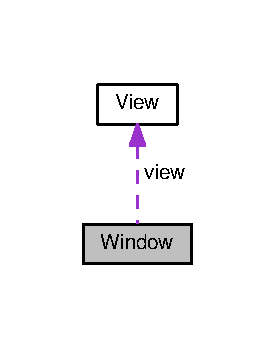
\includegraphics[width=307pt]{classWindow__coll__graph}
\end{center}
\end{figure}
\subsection*{Public Types}
\begin{DoxyCompactItemize}
\item 
\hypertarget{classWindow_a1f4045bbf092073ad31043127af5e27d}{}typedef void(Window\+::$\ast$ {\bfseries thread\+Func}) (void)\label{classWindow_a1f4045bbf092073ad31043127af5e27d}

\end{DoxyCompactItemize}
\subsection*{Public Member Functions}
\begin{DoxyCompactItemize}
\item 
\hyperlink{classWindow_a5996bf7ae672cc3e084d323e4163e4e3}{Window} (\hyperlink{classMyGL}{My\+G\+L} $\ast$parent, int \hyperlink{classWindow_af5b1c436782cc9752d386493fbc5dc8c}{width}, int height, const \hyperlink{structWindowHints}{Window\+Hints} \&wh)
\item 
\hypertarget{classWindow_aad13ee91d93d4033a6e6a8c9cb4ac71f}{}bool {\bfseries handles} (G\+L\+F\+Wwindow $\ast$window)\label{classWindow_aad13ee91d93d4033a6e6a8c9cb4ac71f}

\item 
\hypertarget{classWindow_a4f45493b0f1be74fcee972da50fb8d67}{}void {\bfseries loop} ()\label{classWindow_a4f45493b0f1be74fcee972da50fb8d67}

\item 
\hypertarget{classWindow_a4626829d3cb9d01285f739d2bbc69b74}{}void {\bfseries hide} ()\label{classWindow_a4626829d3cb9d01285f739d2bbc69b74}

\item 
\hypertarget{classWindow_a8f986e19a11c4c97ed8e6ad3d0e648b7}{}void {\bfseries show} ()\label{classWindow_a8f986e19a11c4c97ed8e6ad3d0e648b7}

\item 
\hypertarget{classWindow_a35055c04498121d39741bfcd5082705b}{}void {\bfseries close} ()\label{classWindow_a35055c04498121d39741bfcd5082705b}

\item 
\hypertarget{classWindow_a2132a9fc012c4bbabb0167b027578308}{}void {\bfseries move\+Absolute} (int x, int y)\label{classWindow_a2132a9fc012c4bbabb0167b027578308}

\end{DoxyCompactItemize}
\subsection*{Public Attributes}
\begin{DoxyCompactItemize}
\item 
\hypertarget{classWindow_a9957db4afdad3d57e5c5b6626b44b6d0}{}G\+L\+F\+Wwindow $\ast$ {\bfseries window}\label{classWindow_a9957db4afdad3d57e5c5b6626b44b6d0}

\item 
int \hyperlink{classWindow_af5b1c436782cc9752d386493fbc5dc8c}{width}
\item 
\hypertarget{classWindow_af0ac1732ca6b79a6f6b78aa344140514}{}int {\bfseries height}\label{classWindow_af0ac1732ca6b79a6f6b78aa344140514}

\item 
\hypertarget{classWindow_a76199e6c3402c180d76133da74287f38}{}std\+::unique\+\_\+ptr$<$ std\+::thread $>$ {\bfseries t}\label{classWindow_a76199e6c3402c180d76133da74287f38}

\item 
\hypertarget{classWindow_adb20638db6607fcf6aeb1d06ab6b73f5}{}\hyperlink{classView}{View} $\ast$ {\bfseries current\+View}\label{classWindow_adb20638db6607fcf6aeb1d06ab6b73f5}

\item 
\hypertarget{classWindow_a25bf6f8672c20d053f6f4db8d059fedc}{}std\+::vector$<$ \hyperlink{classView}{View} $\ast$ $>$ {\bfseries views}\label{classWindow_a25bf6f8672c20d053f6f4db8d059fedc}

\item 
\hypertarget{classWindow_a27b66f6aca412b9275fd09d0b203ea78}{}\hyperlink{classMyGL}{My\+G\+L} $\ast$ {\bfseries parent\+My\+G\+L}\label{classWindow_a27b66f6aca412b9275fd09d0b203ea78}

\end{DoxyCompactItemize}


\subsection{Detailed Description}
There may be multiple windows in total. They are all kept track of in the \hyperlink{classMyGL}{My\+G\+L} object. The \hyperlink{classWindow}{Window} class has a function that matches each of the different available glfw callbacks. These functions are registered with glfw in the \hyperlink{classWindow}{Window} constructor. The callback register function accepts a pointer to a G\+L\+F\+Wwindow so I think that these callbacks are window specific. If they weren\textquotesingle{}t window specific then all of the callback functions could be up a level in mygl. The window knows the width and heigth of the screen area in pixels so it is responsible for the pixel\+To\+Real(X/\+Y) functions. It is also responsible for the get\+Cursor\+Pos() function. The window should be responsible for hiding and disabling the mouse cursor. This needs to happen during a pan of the view for example. 

\subsection{Constructor \& Destructor Documentation}
\hypertarget{classWindow_a5996bf7ae672cc3e084d323e4163e4e3}{}\index{Window@{Window}!Window@{Window}}
\index{Window@{Window}!Window@{Window}}
\subsubsection[{Window}]{\setlength{\rightskip}{0pt plus 5cm}Window\+::\+Window (
\begin{DoxyParamCaption}
\item[{{\bf My\+G\+L} $\ast$}]{parent, }
\item[{int}]{width, }
\item[{int}]{height, }
\item[{const {\bf Window\+Hints} \&}]{wh}
\end{DoxyParamCaption}
)}\label{classWindow_a5996bf7ae672cc3e084d323e4163e4e3}
for mac compatability 

\subsection{Member Data Documentation}
\hypertarget{classWindow_af5b1c436782cc9752d386493fbc5dc8c}{}\index{Window@{Window}!width@{width}}
\index{width@{width}!Window@{Window}}
\subsubsection[{width}]{\setlength{\rightskip}{0pt plus 5cm}int Window\+::width}\label{classWindow_af5b1c436782cc9752d386493fbc5dc8c}
The window class needs to know which G\+L\+F\+Wwindow it is taking care of. 1 \hyperlink{classWindow}{Window} for 1 G\+L\+F\+Wwindow 

The documentation for this class was generated from the following files\+:\begin{DoxyCompactItemize}
\item 
My\+G\+L.\+hpp\item 
My\+G\+L.\+cpp\end{DoxyCompactItemize}

\hypertarget{structWindowHints}{}\section{Window\+Hints Struct Reference}
\label{structWindowHints}\index{Window\+Hints@{Window\+Hints}}
\subsection*{Public Attributes}
\begin{DoxyCompactItemize}
\item 
unsigned int {\bfseries glfw\+\_\+context\+\_\+version\+\_\+major}\hypertarget{structWindowHints_a90dcc3c10eff6e9fd9e9731f2098283b}{}\label{structWindowHints_a90dcc3c10eff6e9fd9e9731f2098283b}

\item 
unsigned int {\bfseries glfw\+\_\+context\+\_\+version\+\_\+minor}\hypertarget{structWindowHints_aacea0367d5d087bedca46b89db634963}{}\label{structWindowHints_aacea0367d5d087bedca46b89db634963}

\item 
unsigned int {\bfseries glfw\+\_\+opengl\+\_\+profile}\hypertarget{structWindowHints_afd6fae98a69a4ba82c1c52ef1ea48f36}{}\label{structWindowHints_afd6fae98a69a4ba82c1c52ef1ea48f36}

\item 
unsigned int {\bfseries glfw\+\_\+resizable}\hypertarget{structWindowHints_a0fc16ab2b3016a981bb6983459e68e39}{}\label{structWindowHints_a0fc16ab2b3016a981bb6983459e68e39}

\item 
unsigned int {\bfseries glfw\+\_\+opengl\+\_\+forward\+\_\+compat}\hypertarget{structWindowHints_ac5865247be3897b58f28c094035ea74b}{}\label{structWindowHints_ac5865247be3897b58f28c094035ea74b}

\item 
unsigned int {\bfseries glfw\+\_\+focused}\hypertarget{structWindowHints_a3f9ec495707991985a0105a55e9ab8b4}{}\label{structWindowHints_a3f9ec495707991985a0105a55e9ab8b4}

\item 
unsigned int {\bfseries glfw\+\_\+decorated}\hypertarget{structWindowHints_af8ee369e4bf0d0325f89911bbff4845a}{}\label{structWindowHints_af8ee369e4bf0d0325f89911bbff4845a}

\item 
unsigned int {\bfseries glfw\+\_\+visible}\hypertarget{structWindowHints_a7d5abc43b09c0dec6a87fe0d43cb55aa}{}\label{structWindowHints_a7d5abc43b09c0dec6a87fe0d43cb55aa}

\item 
glm\+::vec4 {\bfseries clear\+Color}\hypertarget{structWindowHints_a740edaeaf708ea2d639b2dbfb488c57c}{}\label{structWindowHints_a740edaeaf708ea2d639b2dbfb488c57c}

\end{DoxyCompactItemize}


The documentation for this struct was generated from the following files\+:\begin{DoxyCompactItemize}
\item 
My\+G\+L.\+hpp\item 
My\+G\+L.\+cpp\end{DoxyCompactItemize}

%--- End generated contents ---

% Index
\backmatter
\newpage
\phantomsection
\clearemptydoublepage
\addcontentsline{toc}{chapter}{Index}
\printindex

\end{document}
